\chapter{Mechanism items and coding scheme for responses}
\label{app:coding}

\section{Materials used by all coders}
\label{sec:materials}

Development of the coding scheme was a multi-step process. Initially, two
members of our group, Sarah Cohen and Roxana Farjadi, saught to identify
conceptions that occurred across multiple surveys. These conceptions were
assigned numerical codes, and these codes were arranged into general categories.
Following this, I developed a more complete progression, describing
relationships between the various categories, as well as grouping them into
“misconceptions,” “ignorance,” and “mechanistic description.” This allowed the
beginnings of a scoring rubric to be developed. We then iterated the process
with a larger group of coders to arrive at the final product reproduced below.
What follows is the full text of the coding packet developed by Ms. Cohen and
Ms. Farjadi, which also contains the text for the mechanism questions we
asked in our interventions. 

Note that \textcite{cohen_san_2012_f} also reports on a coding schema, though
that scheme exhibits differences with the one described here. Following this are
a diagram representing relationships between the codes. A section containing a
set of notes provided by Myles Crain are included in the next section. They
provides a set of criteria for chosing between notes, and was used by the final
set of coders. See chapter~\ref{chap:mechanism} for details.

% Note - there's actually a slightly more up-to-date version of this on google
% docs (edits by Baljeet and me)
\includepdf[pages=-,pagecommand={},landscape=true,scale=.85]%height=6.5in]
           {appendices/coding/codingpacket-blind-Oct26.pdf}

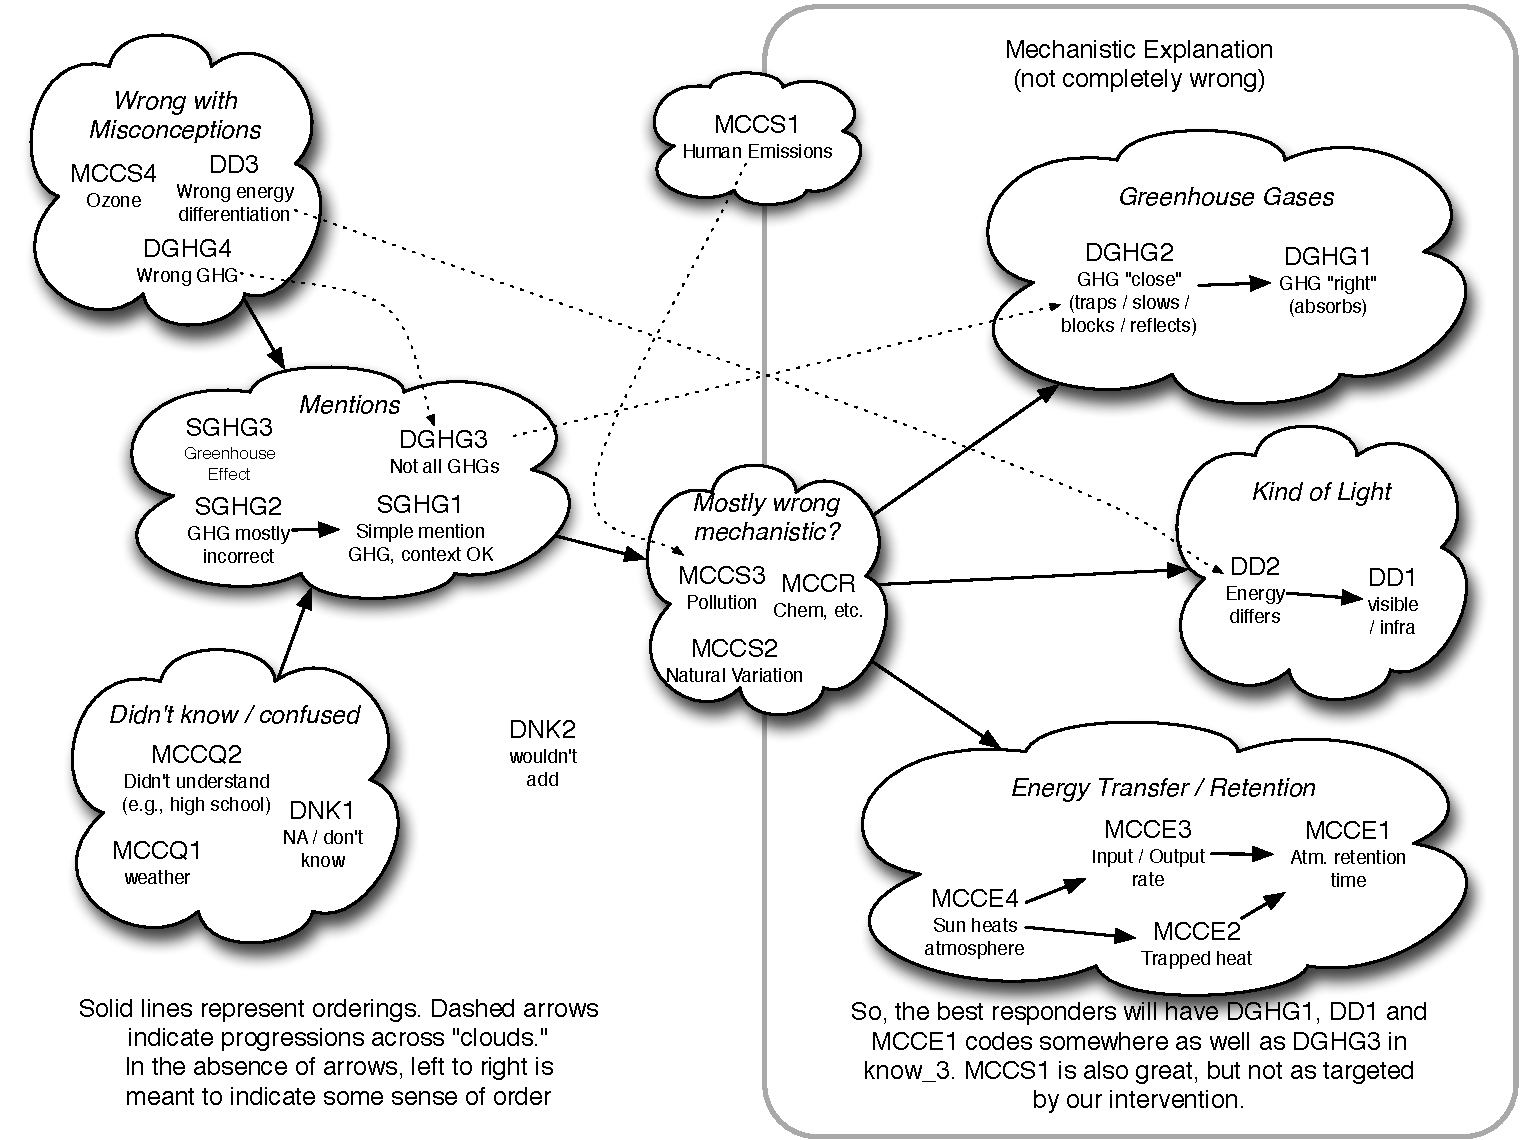
\includepdf[pages=1,pagecommand={},landscape=true,scale=.75]
           {appendices/coding/response-code-progression-letter-codes.pdf}

% Putting this in a landscape environment doesn’t do anything about
% the caption
% Here’s some code from tex.se:
% \begin{landscape} {\includepdf[pages={-},angle=90, offset=8mm 0mm,
% pagecommand={\begin{center}\textbf{~\Cref{fig:label} caption goes
% here.}\end{center}}, addtolist={ 1, caption for TOC goes here,
% tab:label}]{path/to/example.pdf} } \end{landscape}

% \begin{figure}[hp]
% 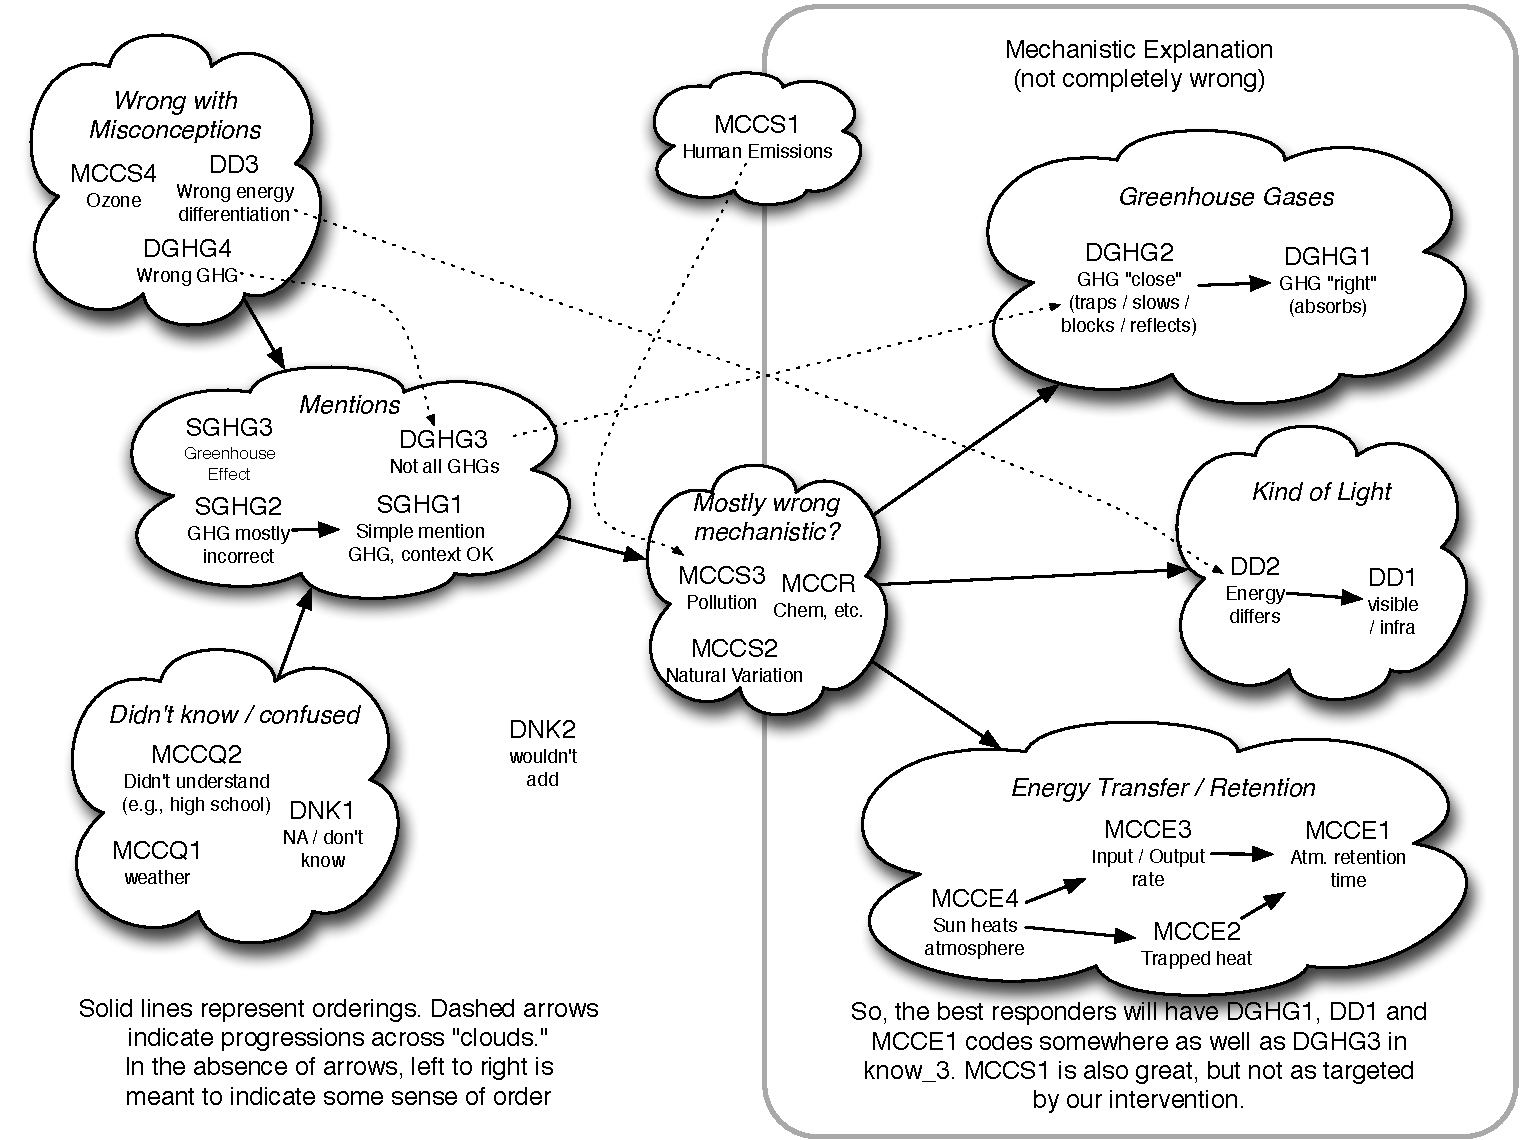
\includegraphics[height=6.5in,angle=90]{appendices/coding/response-code-progression-letter-codes.pdf}
% \caption{“Cloud” Diagram illustrating the relationship between codes}
% \end{figure}

\section{Notes on choosing codes}

This “crib sheet” was generated by Myles Crain to identify a single defining
characteristic and/or unique distinction within each code. Here are a few notes
on how it was used:

\begin{itemize}
\item The crib sheet is NOT self-contained. Its meant to jog memory
without having to constantly flip through the coding packet. The sheet
is only useful if you are generally familiar with the coding scheme
already.

\item Assigning a code should be defensible with explicit references to
the definitions and explanations of that code as provided in the
packet.

\item I've separated DGHG3 from the other DGHG codes intentionally (that
is, DGHG3 coming after DGHG4 is NOT a typo).

\item SGHG codes are only supposed to be used in the complete absence of a
definition of GHGs. The SGHG category is primarily useful in coding
for whether an explanation of climate change includes explicit
reference to GHGs.

\item Use MCCE codes to identify how a participant refers to energy within
an explanation of climate change.

\item Enquoted things are things that must appear in a response in order
to apply the code (except when there are other options--for example,
SGHG1 requires using the phrase "GHG" *or* citing specific examples of
GHGs).
\end{itemize}
Following is the “crib sheet” itself:

\begin{description}
\item[DD1] visible incoming \& infrared outgoing
\item[DD2] asymmetry/difference reference
\item[DD3] wrong, no asymmetry/difference
\vspace{7pt}
\item[DGHG1] GHGs "absorb" energy
\item[DGHG2] part correct, no "absorb"
\item[DGHG4] wrong
\item[DGHG3] "not all", cite >1
\vspace{7pt}
\item[SGHG1] "GHG"/e.g., mostly accurate
\item[SGHG2] "GHG"/e.g., mostly wrong
\item[SGHG3] "greenhouse effect"
\vspace{7pt}
\item[MCCE1] more gas/heat than before
\item[MCCE2] heat/energy "trapped"
\item[MCCE3] different input/output rates/amounts
\item[MCCE4] sun's radiation heats atmosphere
\vspace{7pt}
\item[MCCS1] humans/tech/fossil fuels
\item[MCCS2] natural variation
\item[MCCS3] pollution
\item[MCCS4] O3 layer
\vspace{7pt}
\item[MCCR] chemical/molecular exclusively
\item[MCCQ1] weather, confusion
\item[MCCQ2] irrelevant
\vspace{7pt}
\item[DNK1] "don't know", n/a
\item[DNK2] nothing added
\end{description}

\section{Assigning scores to coded responses}

Detail here the procedure for assigning scores to codes. Perhaps even include
the R or python code?
